\documentclass[a4page]{exam}
\usepackage{geometry}
\usepackage[table]{xcolor}
\usepackage{amsmath, amsfonts}
\usepackage{hyperref}
\usepackage{tikz}
\usetikzlibrary{shapes}
\usetikzlibrary{automata,positioning,arrows}

\tikzset{%
  in place/.style={
    auto=false,
    fill=white,
    inner sep=2pt,
  },
}
% 


\newcommand{\Str}[1]{\mathtt{#1}}
\renewcommand{\a}{\Str{a}}
\renewcommand{\b}{\Str{b}}
\renewcommand{\c}{\Str{c}}

\printanswers

\title{Homework 2}
\author{CS 212 Nature of Computation\\Habib University\\Fall 2021}
\date{Due: 2359h on Sunday, 24 October}

\begin{document}
\maketitle
\thispagestyle{empty}

\noindent\rule{\textwidth}{1pt}

\begin{questions}
\question[10] Prove that $\{wtw | \hspace{1mm} w,t \in \{0,1\}^+\}$ is not regular.

  \begin{solution}
    \textcolor{blue}{Solution taken from the submission by team \textit{pushdown}}.\\
    We can prove this easily using the Pumping Lemma through a proof of contradiction. The pumping lemma states that
    \\If $L$ is a regular language, then there is a number $p$ (the
    pumping length) where if $s$ is any string in L of length at least p, then s may be divided into three pieces, $s = xyz$, satisfying the following conditions:
    \\1. for each $i \geq 0, xy^iz  \in L$,
    \\2. $|y| > 0$, and
    \\3. $|xy| \leq p$

    Let the above language be L. We can assume that s is a string in L of the form $1^p001^p0$
    where p is the pumping length.
    So here, $w = 1^p0$ which is occuring at the beginning and end of the string.
    \\$t=0$ which occurs in the middle of the string. Both of them together form the strings of type $wtw = 1^p0 \;\; 0 \;\; 1^p0$
    The important thing to notice about this choice of string is that w has a clear demarcation of the beginning and the end which implies that if something were to pumped the string might be altered.

    Since $|xy| \leq p$, this implies that $|x| < p$. Since $w = 1^p0$, x and y both must consist of all 1s i.e, $y = 1^l$ where $l>0$ and similarly $x = 1^k$ where $k = p -l$ 

    For pumping, Let $i = 2$ for the 1st clause. $i=2 \rightarrow xy^2z \in  L$. Note that $1^p = 1^{p-l}1^l$. Since y already exists within $1^p$, we only need to add it once more.
    This will result in a string of form $1^{p-l}1^l1^l\;001^p0 = 1^p \;1^l\;001^p0$.
    Simplifying it gives, $1^{p+l}\;001^p0$. There is no way possible in which this string could be split into three parts of the form $wtw$. This is because the 1s on the left handside will always be greater than the 1s on the right part of the string and since the 1s are followed by a single 0 on each end, we will never get the perfect split.This contradicts condition 1 of the pumping lemma stated above. Therefore our assumption of L being a regular language was incorrect. L is not a regular language.
  \end{solution}

\question Given $L = \{0^i1^j2^k | \hspace{1mm} i,j,k \geq 0 \text{ and } i \neq 1 \text{ or } j = k\}$, show that 
  \begin{parts}
  \part[10] $L$ is not regular.
    \begin{solution}
      \textcolor{blue}{Solution taken from the submission by team \textit{pushdown}}.\\
      Apparently, there is no direct way of applying the pumping lemma to this language and proving it non regular. We will use the closure property of regular languages under intersection to show that this language is non regular. 
      The closure property of regular language under intersection on pg 46 of Introduction to the theory of computation states that
      \begin{equation}
        L_1 \text{ is regular } \land L_2 \text{ is regular } \implies L_1 \cap L_2 \text{ is regular }
      \end{equation}
      It's contrapositive would be that
      \begin{equation}
        L_1 \cap L_2 \text{ is non-regular } \implies L_1 \text{ is non-regular } \lor L_2 \text{ is non-regular }
      \end{equation}
      Let us assume that the language $L_1 = \{0^i1^j2^k | \hspace{1mm} i,j,k \geq 0 \text{ and } i \neq 1 \text{ or } j = k\}$ is regular. Let us assume another Language $L_2 = \{ 01^*2^* | \Sigma = \{0,1,2\} \}$
      $L_2$ is regular because the following DFA recognizes it.

      \begin{center}
        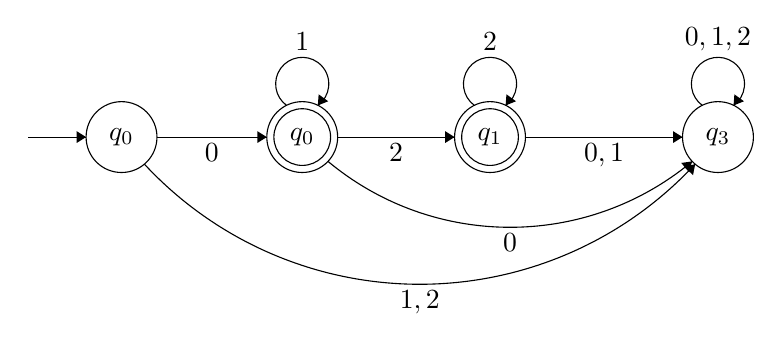
\begin{tikzpicture}[scale=0.15]
          \tikzstyle{every node}+=[inner sep=0pt]
          \draw [black] (28.1,-10.4) circle (3);
          \draw (28.1,-10.4) node {$q_0$};
          \draw [black] (28.1,-10.4) circle (2.4);
          \draw [black] (44,-10.4) circle (3);
          \draw (44,-10.4) node {$q_1$};
          \draw [black] (44,-10.4) circle (2.4);
          \draw [black] (63.3,-10.4) circle (3);
          \draw (63.3,-10.4) node {$q_3$};
          \draw [black] (12.8,-10.4) circle (3);
          \draw (12.8,-10.4) node {$q_0$};
          \draw [black] (26.777,-7.72) arc (234:-54:2.25);
          \draw (28.1,-3.15) node [above] {$1$};
          \fill [black] (29.42,-7.72) -- (30.3,-7.37) -- (29.49,-6.78);
          \draw [black] (42.677,-7.72) arc (234:-54:2.25);
          \draw (44,-3.15) node [above] {$2$};
          \fill [black] (45.32,-7.72) -- (46.2,-7.37) -- (45.39,-6.78);
          \draw [black] (31.1,-10.4) -- (41,-10.4);
          \fill [black] (41,-10.4) -- (40.2,-9.9) -- (40.2,-10.9);
          \draw (36.05,-10.9) node [below] {$2$};
          \draw [black] (47,-10.4) -- (60.3,-10.4);
          \fill [black] (60.3,-10.4) -- (59.5,-9.9) -- (59.5,-10.9);
          \draw (53.65,-10.9) node [below] {$0,1$};
          \draw [black] (61.977,-7.72) arc (234:-54:2.25);
          \draw (63.3,-3.15) node [above] {$0,1,2$};
          \fill [black] (64.62,-7.72) -- (65.5,-7.37) -- (64.69,-6.78);
          \draw [black] (15.8,-10.4) -- (25.1,-10.4);
          \fill [black] (25.1,-10.4) -- (24.3,-9.9) -- (24.3,-10.9);
          \draw (20.45,-10.9) node [below] {$0$};
          \draw [black] (4.9,-10.4) -- (9.8,-10.4);
          \fill [black] (9.8,-10.4) -- (9,-9.9) -- (9,-10.9);
          \draw [black] (61.366,-12.692) arc (-42.85925:-137.14075:31.808);
          \fill [black] (61.37,-12.69) -- (60.46,-12.94) -- (61.19,-13.62);
          \draw (38.05,-23.36) node [below] {$1,2$};
          \draw [black] (61.12,-12.458) arc (-50.20762:-129.79238:24.094);
          \fill [black] (61.12,-12.46) -- (60.19,-12.59) -- (60.83,-13.35);
          \draw (45.7,-18.54) node [below] {$0$};
        \end{tikzpicture}
      \end{center}

      Using the closure property, $L_1 \cap L_2$ will also be regular. 
      \\$L_1 \cap L_2 = (\{0^i1^j2^k | \hspace{1mm} i,j,k \geq 0 \text{ and } i \neq 1 \text{ or } j = k\}) \cap ({01^*2^*})$
      \\Since we are retaining just one 0 in the intersection, the strings in the intersection must have equal 1s and 2s(let's call that number n) in order to exist in $L_1$ i.e, $j=k=n$. Thus the resulting language $L_3 = L_1 \cap L_2 $ will be of the form
      \\$ L_3 = \{ 01^n2^n | n \geq 0 \} $
      Though $L_3$ must be regular, it can be proved that it is non regular using the pumping lemma through a proof of contradiction. The pumping lemma states that
      \\If $L_3$ is a regular language, then there is a number $p$ (the
      pumping length) where if $s$ is any string in A of length at least p, then s may be divided into three pieces, $s = xyz$, satisfying the following conditions:
      \\1. for each $i \geq 0, xy^iz  \in A$,
      \\2. $|y| > 0$, and
      \\3. $|xy| \leq p$

      We can assume that s is a string in the language of the form $01^p2^p$ where p is the pumping length. 
      Since $|xy| \leq p$, this implies that $|x| < p$. Since $s = 01^p2^p$, there can be three possibilities all of which can be pumped to yield strings that do not belong to $L_3$.
      \begin{enumerate}
      \item x can be just $0$ or $01^k$, making $y = 1^l$ where $l>0$. Thus s which is of the form $s = 01^p2^p = 01^{p-l}1^l2^p$, can be pumped up. We set $i=2$, we add one more y. On pumping $1^l$, we will get $s = 01^{p-l}1^l1^l2^p = 01^{p+l}2^p$. Since $l>0$, the number of 1s and 2s become unequal i.e, $p+l \neq p$ hence $s \not \in L_3$ .
      \item x can be empty string $\epsilon$, making $y=01^l$ where $l>0$. On pumping y twice by setting $i=2$, we get $01^{p-l}1^l01^l2^p = 01^p01^l2^p$. This messes up the order of 0 1s and 2s and such $s \not \in L_3$.
      \item x can be empty string and $y=0$ and the rest of the string is $z$.  On pumping y twice by setting $i=2$, we get $001^p2^p$. The number of 0s in the pumped string exceed 1 thus such $s \not \in L_3$.
      \end{enumerate}
      Since no subdivision of $xyz$ exists for which the pumping lemma holds, our assumption of $L_3$ being a regular language was incorrect. Note that the premise of the contrapositive(equation 2) is true. For the implication itself to be true, the consequent must be true. Since we know that $L_2$ is not non-regular because we made a dfa for it, using disjunctive syllogism, $L_1$ must be non regular. This makes the contrapositive true. Hence we have proved that $L_1$ is non regular language.\\\\
    \end{solution}

  \part[10] The pumping lemma for regular languages applies to $L$. That is, show that there is some $p$ such that if $s\in L$ and $|s| > p$, then $s$ can be written as $xyz$ where $|y| > 0, |xy| \le p$, and for each $i \ge 0, xy^iz \in L$.\\ 
    \textit{Note: This shows that the converse of the pumping lemma is false.}
    \begin{solution}
      \textcolor{blue}{Solution adapted from the submission by team \textit{tape}}.\\
      Assuming $p=2$, $s$ can be one of four cases:
      \begin{enumerate}
      \item \underline{$s$ has no zeros $(i = 0)$}: No matter what $xyz$ we take, and how much we pump, $i$ will remain 0, hence resulting string $\in L$.
      \item \underline{$s$ has more than two zeros $(i > 2)$}: We can take $x = \epsilon$ and $y=0$, and then pumping will change $i$, but I will never become 1, so resulting string $\in L$.
      \item \underline{$s$ has one 0 $(i=1)$ and $j=k$}: We can take $x = \epsilon$ and $y=0$, and then regardless of pumping, $j=k$, so resulting string $\in L$.
      \item \underline{$s$ has exactly two 0s $(i = 2)$}: We can take $x = \epsilon$ and $y=00$, and then pumping will change $i$, but I will never become 1, so resulting string $\in L$.        
      \end{enumerate}

      Hence, pumping lemma applies to $L$ for pumping length 2.
    \end{solution}
  \end{parts}

\question Consider the grammar $G = (V,\Sigma, R, S)$ where $V = \{S,A\}$; $\Sigma = \{\a,\b\}$; and $R$ contains the following rules:
  \begin{eqnarray*}
    S &\rightarrow& \a\ A\ \a \mid \b\ A\ \b \mid \epsilon\\
    A &\rightarrow& SS.
  \end{eqnarray*}
  \begin{parts}
  \part[5] Which strings of $L(G)$ can be produced by derivations of four or fewer steps?
  \part[5] Give a derivation of $\Str{baabbb}$ in $G$.
  \part[5] Construct the parse tree of the derivation from the previous part.
  \part[5] Describe $L(G)$ in English?
  \end{parts}

  \begin{solution}{}
    \textcolor{blue}{Solution taken from the submission by team \textit{prefix}}.
    \begin{parts}
    \part Consider deriving a string, $w$ where $|w|>0$ from $A$ in minimum number of steps\\
      $A $\\
      $\rightarrow SS $\\
      $\rightarrow \Str{a}\ A\ \Str{a} \ S $\\
      $\rightarrow \Str{a}\ A\ \Str{a} $\\
      $\rightarrow \Str{a}\ SS\ \Str{a} $\\
      $\rightarrow \Str{a}\ S\ \Str{a} $\\
      $\rightarrow \Str{a} \Str{a} $\\

      $A $\\
      $\rightarrow SS $\\
      $\rightarrow \Str{b}\ A\ \Str{b} \ S $\\
      $\rightarrow \Str{b}\ A\ \Str{b} $\\
      $\rightarrow \Str{b}\ SS\ \Str{b} $\\
      $\rightarrow \Str{b}\ S\ \Str{b} $\\
      $\rightarrow \Str{b} \Str{b} $\\

      Therefore the minimum number of steps required to derive a string $w$ where $|w|>0$ is 6.
      As these number of steps are more than 4, substitutions with $A$ can only be made to yield the empty string, 
      if we want to derive in less than 4 steps

      $S \rightarrow \Str{a}\ A\ \Str{a} \mid \Str{b}\ A\ \Str{b} \mid \epsilon$\\

      Therefore possible derivations in 4 steps are:

      \quad $S \rightarrow \Str{a}\ A\ \Str{a} \rightarrow \Str{a}\ SS\ \Str{a} \rightarrow \Str{a}\ S\ \Str{a} \rightarrow aa$

      \quad $S \rightarrow \Str{b}\ A\ \Str{b} \rightarrow \Str{b}\ SS\ \Str{b} \rightarrow \Str{b}\ S\ \Str{b} \rightarrow bb$ 

      \quad $S \rightarrow \epsilon $

      Note derivations with same result from a derivation already present have been omitted

      So possible strings that can be produced in 4 steps are $aa$, $bb$, and $\epsilon$.
    \part $S \rightarrow \Str{b}\ A\ \Str{b} \rightarrow \Str{b}\ SS\ \Str{b} \rightarrow \Str{b} \Str{a}\ A\ \Str{a} \ S \ \Str{b} \rightarrow \Str{b} \Str{a}\ SS\ \Str{a} \ S \ \Str{b} \rightarrow \Str{b} \Str{a}\ S\ \Str{a} \ S \ \Str{b} \rightarrow \Str{b} \Str{a}\Str{a} \ S \ \Str{b}$\\
      $\rightarrow \Str{b} \Str{a}\Str{a} \Str{b}\ A\ \Str{b} \Str{b} \rightarrow \Str{b} \Str{a}\Str{a} \Str{b}\ SS\ \Str{b} \Str{b} \rightarrow \Str{b} \Str{a}\Str{a} \Str{b} \ S\ \Str{b} \Str{b} \rightarrow \Str{b} \Str{a}\Str{a} \Str{b} \Str{b} \Str{b}$\\

    \part \ \\
      
      \begin{tikzpicture}[font=\sffamily,thick,level/.style={sibling distance=40mm/#1}]
        \node {S}
        child {
          node {b}
        }
        child {
          node {A}
          child {
            node{S}
            child { 
              node {a} }
            child {
              node {A}
              child { 
                node{S}
                child {
                  node{$\varepsilon$}
                }
              }
              child { 
                node{S}
                child {
                  node{$\varepsilon$}
                }
              }
            }
            child { 
              node {a} }
          }
          child {
            node{S}
            child { 
              node {a} }
            child {
              node {A}
              child { 
                node{S}
                child {
                  node{$\varepsilon$}
                }
              }
              child { 
                node{S}
                child {
                  node{$\varepsilon$}
                }
              }
            }
            child { 
              node {a} }
          }
        } 
        child {
          node {b}
        }
        ;
      \end{tikzpicture}


    \part L(G) are all strings consisting of $a$ and $b$ where each letter in the string can be matched to another same letter in the string with
      an even number of letters between the two letters
    \end{parts}
  \end{solution}
  
\question[10] Convert the following context-free grammar to Chomsky Normal Form:
  \begin{eqnarray*}
    S &\rightarrow& A\ S\ B\\
    A &\rightarrow& \a\ A\ S\ \mid\  \a\ \mid\ \epsilon \\
    B &\rightarrow& S\ \b\ S\ \mid\ A\ \mid\ \b\ \b.
  \end{eqnarray*}

  \begin{solution}
    \textcolor{blue}{Solution by WS}.
    \begin{eqnarray*}
      S_0 &\rightarrow& A\ U\ \mid\ A\ S\ \mid\ S\ B \\
      S &\rightarrow& A\ U\ \mid\ A\ S\ \mid\ S\ B \\
      A &\rightarrow& W\ V\ \mid\ W\ S\ \mid\  \a \\
      B &\rightarrow& S\ Y\ \mid\ W\ V\ \mid\ W\ S\ \mid\  \a\ \mid\ X\ X\\
      U &\rightarrow& S\ B\\
      V &\rightarrow& A\ S\\
      W &\rightarrow& \a\\
      X &\rightarrow& \b\\
      Y &\rightarrow& X\ S\\
    \end{eqnarray*}

  \end{solution}
  
\question Give an unambiguous context-free grammar and then construct a pushdown automaton for each of the following languages.
  \begin{parts}
  \part[20] $L = \{\a^n \b^m \c^k \mid n, m, k > 0, k = n + m \}$ over $\Sigma = \{\a, \b, \c\}$.
    
    \begin{solution}
      \textcolor{blue}{Solution by WS}.
      \paragraph{CFG:} Member strings can be viewed as $\textcolor{blue}{\a^n}\textcolor{red}{\b^m\c^m}\textcolor{blue}{\c^n}$. $S$ below generates the blue part of the string and hands over to $T$ to generate the embedded red part.
      \begin{eqnarray*}
        S &\rightarrow& \a\ S\ \c\ \mid\ \a\ T\ \c\\
        T &\rightarrow& \b\ T\ \c\ \mid\ \b\ \c\\
      \end{eqnarray*}
      
      \paragraph{PDA:} The transition function of the corresponding PDA is shown below. It uses the shorthand from the book for transitions corresponding to rule productions.

      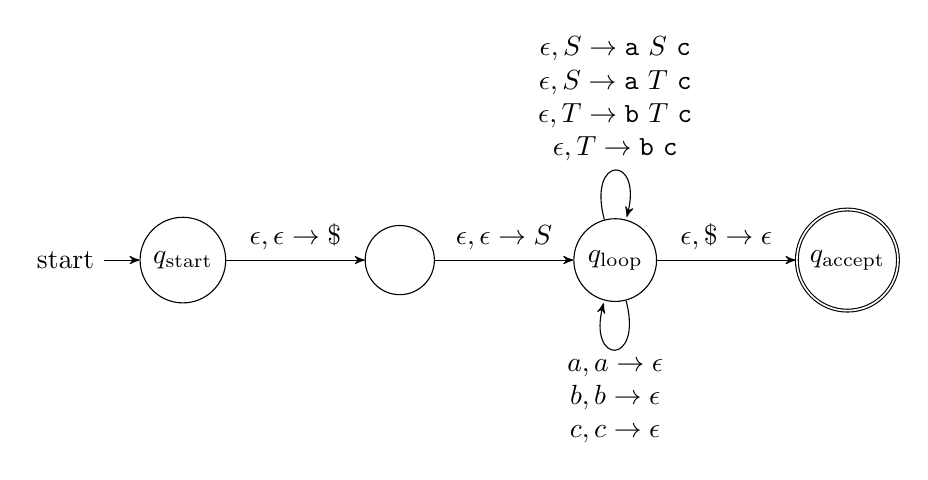
\begin{tikzpicture}[auto, ->,>=stealth',node distance=50pt]
        \node[state,initial] (q_0) {$q_{\text{start}}$};
        \node[state] (q_1) [right = of q_0] {};
        \node[state] (q_2) [right = of q_1] {$q_{\text{loop}}$};
        \node[state,accepting] (q_3) [right = of q_2] {$q_{\text{accept}}$};

        \path (q_0) edge              node [above] {$\epsilon, \epsilon \rightarrow \$$} (q_1)
        (q_1) edge              node [above] {$\epsilon, \epsilon \rightarrow S$} (q_2)
        (q_2) edge [loop above] node [align=center] {
          $\epsilon, S \rightarrow \a\ S\ \c$\\
          $\epsilon, S \rightarrow \a\ T\ \c$\\
          $\epsilon, T \rightarrow \b\ T\ \c$\\
          $\epsilon, T \rightarrow \b\ \c$
        } (q_2)
        (q_2) edge [loop below] node [align=center] {
          $a, a \rightarrow \epsilon$\\
          $b, b \rightarrow \epsilon$\\
          $c, c \rightarrow \epsilon$
        } (q_2)
        (q_2) edge              node [above] {$\epsilon, \$ \rightarrow \epsilon$} (q_3);
      \end{tikzpicture}
      
    \end{solution}
    
  \part[20] $A = \{w \mid \text{the number of $\a$'s is at least the number of $\b$'s in $w$} \}$ over $\Sigma = \{\a, \b\}$.
    
    \begin{solution}
      \textcolor{blue}{Solution by WS}.
      \paragraph{CFG:} Member strings can be categorized as follows. Some strings contain an equal number of $\a$'s and $\b$'s. Let's call these \textit{balanced} strings. Others contain more $\a$'s than $\b$'s. These are balanced strings with excess $\a$'s. This yields a grammar like the following.
      \begin{eqnarray*}
        S &\rightarrow& \a\ S\ \b\ \mid\ \b\ S\ \a\ \mid\ S\ S\ \mid\ \a\ \mid\ \epsilon
      \end{eqnarray*}
      But this grammar is ambiguous, e.g. multiple derivations of $a$. An unambiguous grammar is more complicated to achieve. A graphical explanation is given \href{https://cs.stackexchange.com/questions/125516/unambiguous-context-free-grammar-for-strings-with-at-least-as-many-as-as-bs}{here} which yields the following grammar.
      \begin{eqnarray*}
        S & \rightarrow & S\ \a\ U\ \mid\ X\\
	X & \rightarrow & \a\ U\ \b\ X\ \mid\ \b\ D\ \a\ X\ \mid\ \epsilon\\
        D & \rightarrow & \b\ D\ \a\ D\ \mid\ \epsilon\\
        U & \rightarrow & \a\ U\ \b\ U\ \mid\ \epsilon
      \end{eqnarray*}
      
      \paragraph{PDA:} The transition function of the corresponding PDA is shown below. It uses the shorthand from the book for transitions corresponding to rule productions.

      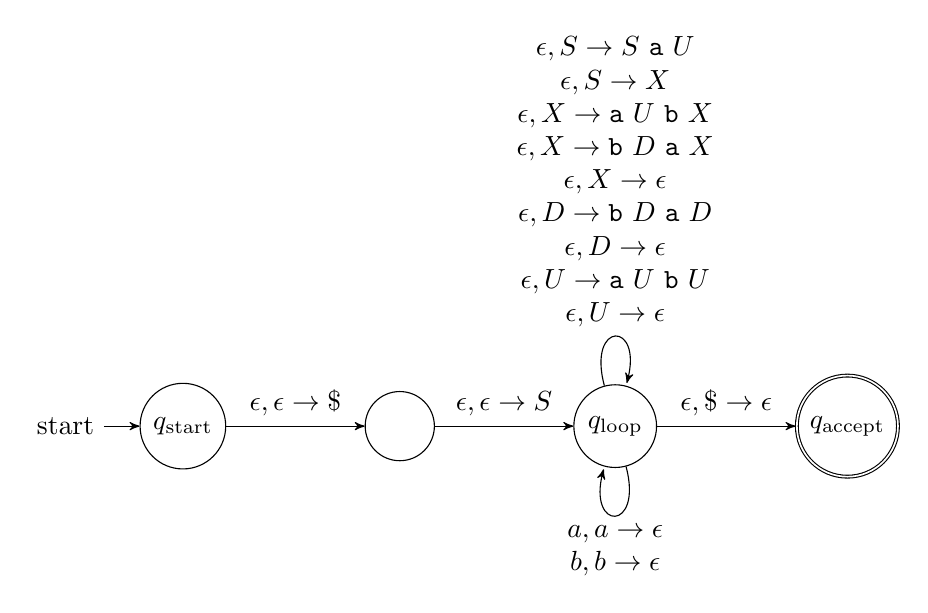
\begin{tikzpicture}[auto, ->,>=stealth',node distance=50pt]
        \node[state,initial] (q_0) {$q_{\text{start}}$};
        \node[state] (q_1) [right = of q_0] {};
        \node[state] (q_2) [right = of q_1] {$q_{\text{loop}}$};
        \node[state,accepting] (q_3) [right = of q_2] {$q_{\text{accept}}$};

        \path (q_0) edge              node [above] {$\epsilon, \epsilon \rightarrow \$$} (q_1)
        (q_1) edge              node [above] {$\epsilon, \epsilon \rightarrow S$} (q_2)
        (q_2) edge [loop above] node [align=center] {
          $\epsilon, S \rightarrow S\ \a\ U$\\
          $\epsilon, S \rightarrow X$\\
          $\epsilon, X \rightarrow \a\ U\ \b\ X$\\
          $\epsilon, X \rightarrow \b\ D\ \a\ X$\\
          $\epsilon, X \rightarrow \epsilon$\\
          $\epsilon, D \rightarrow \b\ D\ \a\ D$\\
          $\epsilon, D \rightarrow \epsilon$\\
          $\epsilon, U \rightarrow \a\ U\ \b\ U$\\
          $\epsilon, U \rightarrow \epsilon$
        } (q_2)
        (q_2) edge [loop below] node [align=center] {
          $a, a \rightarrow \epsilon$\\
          $b, b \rightarrow \epsilon$
        } (q_2)
        (q_2) edge              node [above] {$\epsilon, \$ \rightarrow \epsilon$} (q_3);
      \end{tikzpicture}
    \end{solution}
  \end{parts}
  
\end{questions}

\noindent\rule{\textwidth}{1pt}
\end{document}

%%% Local Variables:
%%% mode: latex
%%% TeX-master: t
%%% End:
